\documentclass{standalone}
\usepackage{tikz}
\usetikzlibrary{patterns, positioning}

\begin{document}
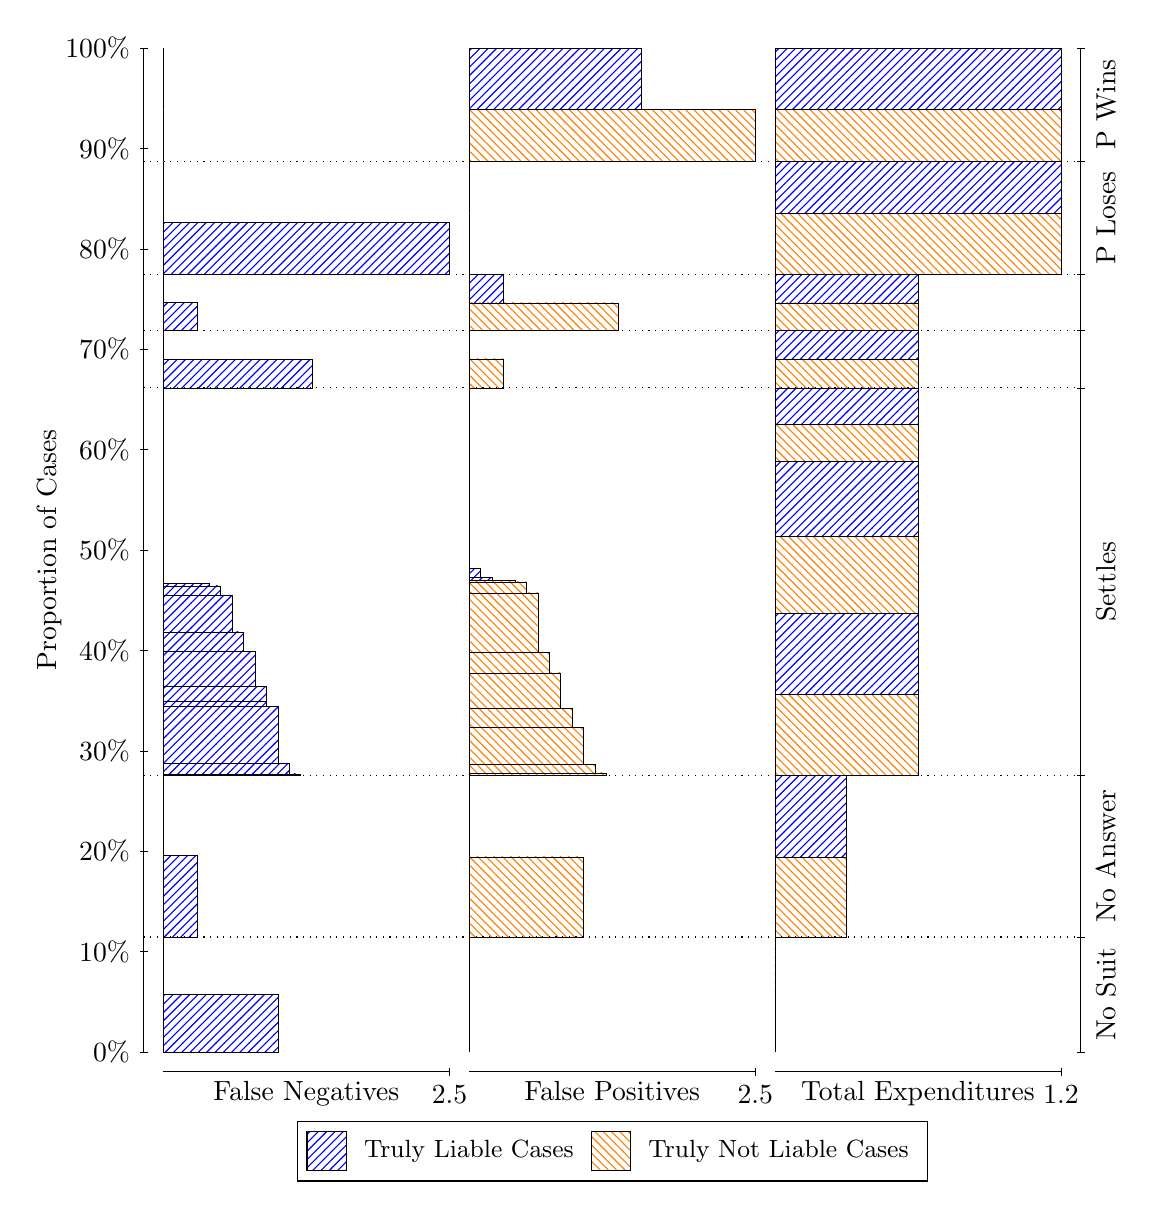
\begin{tikzpicture}
\draw[black, very thin] (1.5,1.75) -- (1.5,14.5);
\node[rotate=90, anchor=center] at (0.3, 8.125) {Proportion of Cases};
\draw[black, very thin] (1.45,1.75) -- (1.55,1.75);
\node[anchor=east] at (1.45, 1.75) {0\%};
\draw[black, very thin] (1.45,3.025) -- (1.55,3.025);
\node[anchor=east] at (1.45, 3.025) {10\%};
\draw[black, very thin] (1.45,4.3) -- (1.55,4.3);
\node[anchor=east] at (1.45, 4.3) {20\%};
\draw[black, very thin] (1.45,5.575) -- (1.55,5.575);
\node[anchor=east] at (1.45, 5.575) {30\%};
\draw[black, very thin] (1.45,6.85) -- (1.55,6.85);
\node[anchor=east] at (1.45, 6.85) {40\%};
\draw[black, very thin] (1.45,8.125) -- (1.55,8.125);
\node[anchor=east] at (1.45, 8.125) {50\%};
\draw[black, very thin] (1.45,9.4) -- (1.55,9.4);
\node[anchor=east] at (1.45, 9.4) {60\%};
\draw[black, very thin] (1.45,10.675) -- (1.55,10.675);
\node[anchor=east] at (1.45, 10.675) {70\%};
\draw[black, very thin] (1.45,11.95) -- (1.55,11.95);
\node[anchor=east] at (1.45, 11.95) {80\%};
\draw[black, very thin] (1.45,13.225) -- (1.55,13.225);
\node[anchor=east] at (1.45, 13.225) {90\%};
\draw[black, very thin] (1.45,14.5) -- (1.55,14.5);
\node[anchor=east] at (1.45, 14.5) {100\%};

\draw[black, very thin] (13.4,1.75) -- (13.4,14.5);
\draw[black, very thin] (13.35,1.75) -- (13.45,1.75);
\node[anchor=west] at (13.35, 1.75) {};
\draw[black, very thin] (13.35,3.2105) -- (13.45,3.2105);
\node[anchor=west] at (13.35, 3.2105) {};
\draw[black, very thin] (13.35,5.2602) -- (13.45,5.2602);
\node[anchor=west] at (13.35, 5.2602) {};
\draw[black, very thin] (13.35,10.184) -- (13.45,10.184);
\node[anchor=west] at (13.35, 10.184) {};
\draw[black, very thin] (13.35,10.911) -- (13.45,10.911);
\node[anchor=west] at (13.35, 10.911) {};
\draw[black, very thin] (13.35,11.622) -- (13.45,11.622);
\node[anchor=west] at (13.35, 11.622) {};
\draw[black, very thin] (13.35,13.06) -- (13.45,13.06);
\node[anchor=west] at (13.35, 13.06) {};
\draw[black, very thin] (13.35,14.5) -- (13.45,14.5);
\node[anchor=west] at (13.35, 14.5) {};

\draw[black, very thin, pattern color=blue, pattern=north east lines] (1.75,1.75) rectangle (3.2033,2.4853);
\draw[black, very thin, pattern color=orange, pattern=north west lines] (1.75,2.4853) rectangle (1.75,3.2105);
\draw[black, very thin, pattern color=blue, pattern=north east lines] (1.75,3.2105) rectangle (2.186,4.2423);
\draw[black, very thin, pattern color=orange, pattern=north west lines] (1.75,4.2423) rectangle (1.75,5.2602);
\draw[black, very thin, pattern color=blue, pattern=north east lines] (1.75,5.2602) rectangle (3.494,5.2807);
\draw[black, very thin, pattern color=blue, pattern=north east lines] (1.75,5.2807) rectangle (3.3487,5.4122);
\draw[black, very thin, pattern color=blue, pattern=north east lines] (1.75,5.4122) rectangle (3.2033,6.1431);
\draw[black, very thin, pattern color=blue, pattern=north east lines] (1.75,6.1431) rectangle (3.058,6.2086);
\draw[black, very thin, pattern color=blue, pattern=north east lines] (1.75,6.2086) rectangle (3.058,6.3973);
\draw[black, very thin, pattern color=blue, pattern=north east lines] (1.75,6.3973) rectangle (2.9127,6.8417);
\draw[black, very thin, pattern color=blue, pattern=north east lines] (1.75,6.8417) rectangle (2.7673,7.0845);
\draw[black, very thin, pattern color=blue, pattern=north east lines] (1.75,7.0845) rectangle (2.622,7.551);
\draw[black, very thin, pattern color=blue, pattern=north east lines] (1.75,7.551) rectangle (2.4767,7.6686);
\draw[black, very thin, pattern color=blue, pattern=north east lines] (1.75,7.6686) rectangle (2.3313,7.7037);
\draw[black, very thin, pattern color=orange, pattern=north west lines] (1.75,7.7037) rectangle (1.75,10.184);
\draw[black, very thin, pattern color=blue, pattern=north east lines] (1.75,10.184) rectangle (3.6393,10.544);
\draw[black, very thin, pattern color=orange, pattern=north west lines] (1.75,10.544) rectangle (1.75,10.911);
\draw[black, very thin, pattern color=blue, pattern=north east lines] (1.75,10.911) rectangle (2.186,11.271);
\draw[black, very thin, pattern color=orange, pattern=north west lines] (1.75,11.271) rectangle (1.75,11.622);
\draw[black, very thin, pattern color=blue, pattern=north east lines] (1.75,11.622) rectangle (5.3833,12.285);
\draw[black, very thin, pattern color=orange, pattern=north west lines] (1.75,12.285) rectangle (1.75,13.06);
\draw[black, very thin, pattern color=orange, pattern=north west lines] (1.75,13.06) rectangle (1.75,13.719);
\draw[black, very thin, pattern color=blue, pattern=north east lines] (1.75,13.719) rectangle (1.75,14.5);
\draw[black, very thin, pattern color=orange, pattern=north west lines] (5.6333,1.75) rectangle (5.6333,2.4752);
\draw[black, very thin, pattern color=blue, pattern=north east lines] (5.6333,2.4752) rectangle (5.6333,3.2105);
\draw[black, very thin, pattern color=orange, pattern=north west lines] (5.6333,3.2105) rectangle (7.0867,4.2284);
\draw[black, very thin, pattern color=blue, pattern=north east lines] (5.6333,4.2284) rectangle (5.6333,5.2602);
\draw[black, very thin, pattern color=orange, pattern=north west lines] (5.6333,5.2602) rectangle (7.3773,5.2934);
\draw[black, very thin, pattern color=orange, pattern=north west lines] (5.6333,5.2934) rectangle (7.232,5.4061);
\draw[black, very thin, pattern color=orange, pattern=north west lines] (5.6333,5.4061) rectangle (7.0867,5.87);
\draw[black, very thin, pattern color=orange, pattern=north west lines] (5.6333,5.87) rectangle (6.9413,6.1109);
\draw[black, very thin, pattern color=orange, pattern=north west lines] (5.6333,6.1109) rectangle (6.796,6.5655);
\draw[black, very thin, pattern color=orange, pattern=north west lines] (5.6333,6.5655) rectangle (6.6507,6.8296);
\draw[black, very thin, pattern color=orange, pattern=north west lines] (5.6333,6.8296) rectangle (6.5053,7.5807);
\draw[black, very thin, pattern color=orange, pattern=north west lines] (5.6333,7.5807) rectangle (6.36,7.7192);
\draw[black, very thin, pattern color=orange, pattern=north west lines] (5.6333,7.7192) rectangle (6.2147,7.7407);
\draw[black, very thin, pattern color=blue, pattern=north east lines] (5.6333,7.7407) rectangle (5.924,7.7758);
\draw[black, very thin, pattern color=blue, pattern=north east lines] (5.6333,7.7758) rectangle (5.7787,7.8933);
\draw[black, very thin, pattern color=blue, pattern=north east lines] (5.6333,7.8933) rectangle (5.6333,10.184);
\draw[black, very thin, pattern color=orange, pattern=north west lines] (5.6333,10.184) rectangle (6.0693,10.551);
\draw[black, very thin, pattern color=blue, pattern=north east lines] (5.6333,10.551) rectangle (5.6333,10.911);
\draw[black, very thin, pattern color=orange, pattern=north west lines] (5.6333,10.911) rectangle (7.5227,11.262);
\draw[black, very thin, pattern color=blue, pattern=north east lines] (5.6333,11.262) rectangle (6.0693,11.622);
\draw[black, very thin, pattern color=orange, pattern=north west lines] (5.6333,11.622) rectangle (5.6333,12.396);
\draw[black, very thin, pattern color=blue, pattern=north east lines] (5.6333,12.396) rectangle (5.6333,13.06);
\draw[black, very thin, pattern color=orange, pattern=north west lines] (5.6333,13.06) rectangle (9.2667,13.719);
\draw[black, very thin, pattern color=blue, pattern=north east lines] (5.6333,13.719) rectangle (7.8133,14.5);
\draw[black, very thin, pattern color=orange, pattern=north west lines] (9.5167,1.75) rectangle (9.5167,2.4752);
\draw[black, very thin, pattern color=blue, pattern=north east lines] (9.5167,2.4752) rectangle (9.5167,3.2105);
\draw[black, very thin, pattern color=orange, pattern=north west lines] (9.5167,3.2105) rectangle (10.425,4.2284);
\draw[black, very thin, pattern color=blue, pattern=north east lines] (9.5167,4.2284) rectangle (10.425,5.2602);
\draw[black, very thin, pattern color=orange, pattern=north west lines] (9.5167,5.2602) rectangle (11.333,6.2913);
\draw[black, very thin, pattern color=blue, pattern=north east lines] (9.5167,6.2913) rectangle (11.333,7.3197);
\draw[black, very thin, pattern color=orange, pattern=north west lines] (9.5167,7.3197) rectangle (11.333,8.2999);
\draw[black, very thin, pattern color=blue, pattern=north east lines] (9.5167,8.2999) rectangle (11.333,9.2482);
\draw[black, very thin, pattern color=orange, pattern=north west lines] (9.5167,9.2482) rectangle (11.333,9.7175);
\draw[black, very thin, pattern color=blue, pattern=north east lines] (9.5167,9.7175) rectangle (11.333,10.184);
\draw[black, very thin, pattern color=orange, pattern=north west lines] (9.5167,10.184) rectangle (11.333,10.551);
\draw[black, very thin, pattern color=blue, pattern=north east lines] (9.5167,10.551) rectangle (11.333,10.911);
\draw[black, very thin, pattern color=orange, pattern=north west lines] (9.5167,10.911) rectangle (11.333,11.262);
\draw[black, very thin, pattern color=blue, pattern=north east lines] (9.5167,11.262) rectangle (11.333,11.622);
\draw[black, very thin, pattern color=orange, pattern=north west lines] (9.5167,11.622) rectangle (13.15,12.396);
\draw[black, very thin, pattern color=blue, pattern=north east lines] (9.5167,12.396) rectangle (13.15,13.06);
\draw[black, very thin, pattern color=orange, pattern=north west lines] (9.5167,13.06) rectangle (13.15,13.719);
\draw[black, very thin, pattern color=blue, pattern=north east lines] (9.5167,13.719) rectangle (13.15,14.5);
\draw[black, dotted] (1.5,3.2105) -- (13.4,3.2105);
\draw[black, dotted] (1.5,5.2602) -- (13.4,5.2602);
\draw[black, dotted] (1.5,10.184) -- (13.4,10.184);
\draw[black, dotted] (1.5,10.911) -- (13.4,10.911);
\draw[black, dotted] (1.5,11.622) -- (13.4,11.622);
\draw[black, dotted] (1.5,13.06) -- (13.4,13.06);
\draw[black, very thin] (1.75,1.5) -- (5.3833,1.5);
\node[anchor=north] at (3.5667, 1.5) {False Negatives};
\draw[black, very thin] (5.3833,1.45) -- (5.3833,1.55);
\node[anchor=north] at (5.3833, 1.45) {2.5};

\draw[black, very thin] (5.6333,1.5) -- (9.2667,1.5);
\node[anchor=north] at (7.45, 1.5) {False Positives};
\draw[black, very thin] (9.2667,1.45) -- (9.2667,1.55);
\node[anchor=north] at (9.2667, 1.45) {2.5};

\draw[black, very thin] (9.5167,1.5) -- (13.15,1.5);
\node[anchor=north] at (11.333, 1.5) {Total Expenditures};
\draw[black, very thin] (13.15,1.45) -- (13.15,1.55);
\node[anchor=north] at (13.15, 1.45) {1.2};

\node[black, centered, rotate=90] at (13.72, 2.4802) {No Suit};
\node[black, centered, rotate=90] at (13.72, 4.2353) {No Answer};
\node[black, centered, rotate=90] at (13.72, 7.7222) {Settles};


\node[black, centered, rotate=90] at (13.72, 12.341) {P Loses};
\node[black, centered, rotate=90] at (13.72, 13.78) {P Wins};

\draw (7.449999999999999,1.5) node[draw=none] (baseCoordinate) {};
\begin{scope}[align=center]
        \matrix[scale=0.5, draw=black, below=0.5cm of baseCoordinate, nodes={draw}, column sep=0.1cm]{
            \node[rectangle, draw, minimum width=0.5cm, minimum height=0.5cm, pattern=north east lines, pattern color=blue] {}; &
            \node[draw=none, font=\small] (B) {Truly Liable Cases}; &
            \node[rectangle, draw, minimum width=0.5cm, minimum height=0.5cm, pattern=north west lines, pattern color=orange] {}; &
            \node[draw=none, font=\small] (B) {Truly Not Liable Cases}; \\
            };
\end{scope}

\end{tikzpicture}
\end{document}